\chapter {Performance Analysis}
\label{chap:result}
As we have described the proposed method in the chapter \ref{chap:algorithm}. In this chapter we will discuss about result and performance.
\section{Environments of Experiments}
Text examples in public datasets usually occur within high-quality (high-resolution, well-focused) imagery. In our setting, text often occurs at lower-resolution and with significant blur. Our focus is to achieve text spotting in a real-time system moving through an environment. We first examine how much the information is attached with an analogue image than we detect the text and extract the data. Next, we train the data. Finally, we evaluate the accuracy.
We tested with many different categories of the images such as images are taken with mobile camera, scanning images, DSLR camera and handy cam. The accuracy of the output varied greatly. Accuracy varies mainly for image quality. An image is taken with DSLR camera produces most accurate results for it's picture quality. Image of DSLR camera is less noise free. So, it’s easy to extract data and OCR can detect the data perfectly. For handy cam images accuracy is slightly get down. Because picture quality is not good as DSLR camera and there is more noise.
If we use scanned images, it it produces more accurate result than handy cam. Because there is less noise than handy cam images. But for mobile camera images the accuracy level is not so good as regarding the other three image categories. For mobile camera there is more noise and image quality is not good.   

\section{Performance for English form}
We test our proposed algorithm in different types of sample form. The result depends on the tesseract training data. For english we train "Arial","Courier","Calibri","Times New Roman" fonts. Here we show our some output result and analysis of our training data.
\subsection{English Sample form 1}

\begin{figure}[H]
\centering
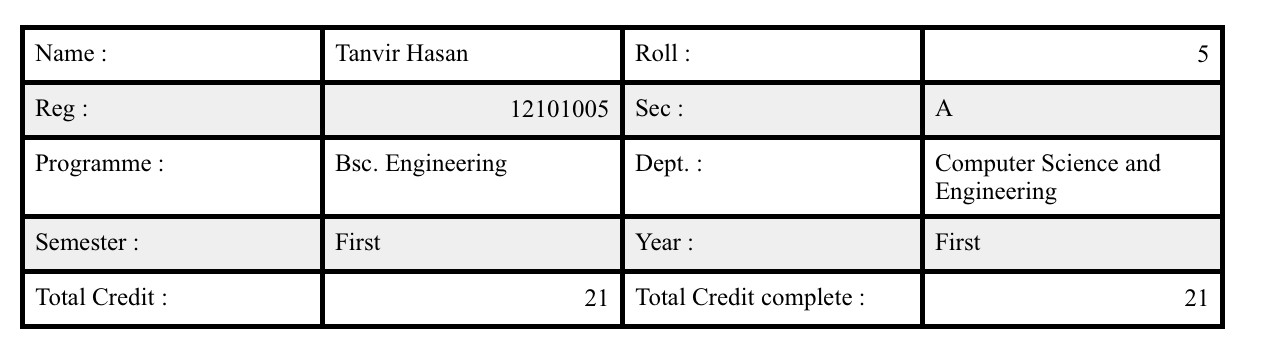
\includegraphics[width=1\textwidth]{form1.png}
\caption {Sample English form 1}
\label {fig:form1}
\end{figure}

\begin{table}[H]
\centering
\begin{tabular}{|p{2cm}|p{2cm}|p{2cm}|}
\hline
character & Input Frequency & Output Frequency \\
\hline
. & 1 & 0\\
\hline
1 & 5 & 7\\
\hline
0 & 3 & 3\\
\hline
2 & 3 & 3\\
\hline
5 & 2 & 2\\
\hline
8 & 0 & 4\\
\hline
: & 10 & 10\\
\hline
A & 1 & 1\\
\hline
C & 3 & 3\\
\hline
B & 1 & 1\\
\hline
E & 2 & 1\\
\hline
D & 1 & 1\\
\hline
F & 2 & 2\\
\hline
I & 0 & 2\\
\hline
H & 1 & 2\\
\hline
N & 1 & 1\\
\hline
P & 1 & 1\\
\hline
S & 3 & 3\\
\hline
R & 2 & 2\\
\hline
T & 3 & 3\\
\hline
Y & 1 & 2\\
\hline
a & 10 & 9\\
\hline
c & 5 & 5\\
\hline
e & 20 & 18\\
\hline
d & 3 & 3\\
\hline
g & 6 & 0\\
\hline
i & 10 & 8\\
\hline
m & 6 & 6\\
\hline
l & 6 & 1\\
\hline
o & 6 & 6\\
\hline
n & 11 & 7\\
\hline
p & 3 & 3\\
\hline
s & 4 & 5\\
\hline
r & 11 & 11\\
\hline
u & 1 & 1\\
\hline
t & 9 & 10\\
\hline
v & 1 & 1\\
\hline
\end{tabular}
\caption { Comparison between Input and Output frequency of English Sample Input 1}
\label {tab:Table1}
\end{table}

\begin{figure}[H]
\centering
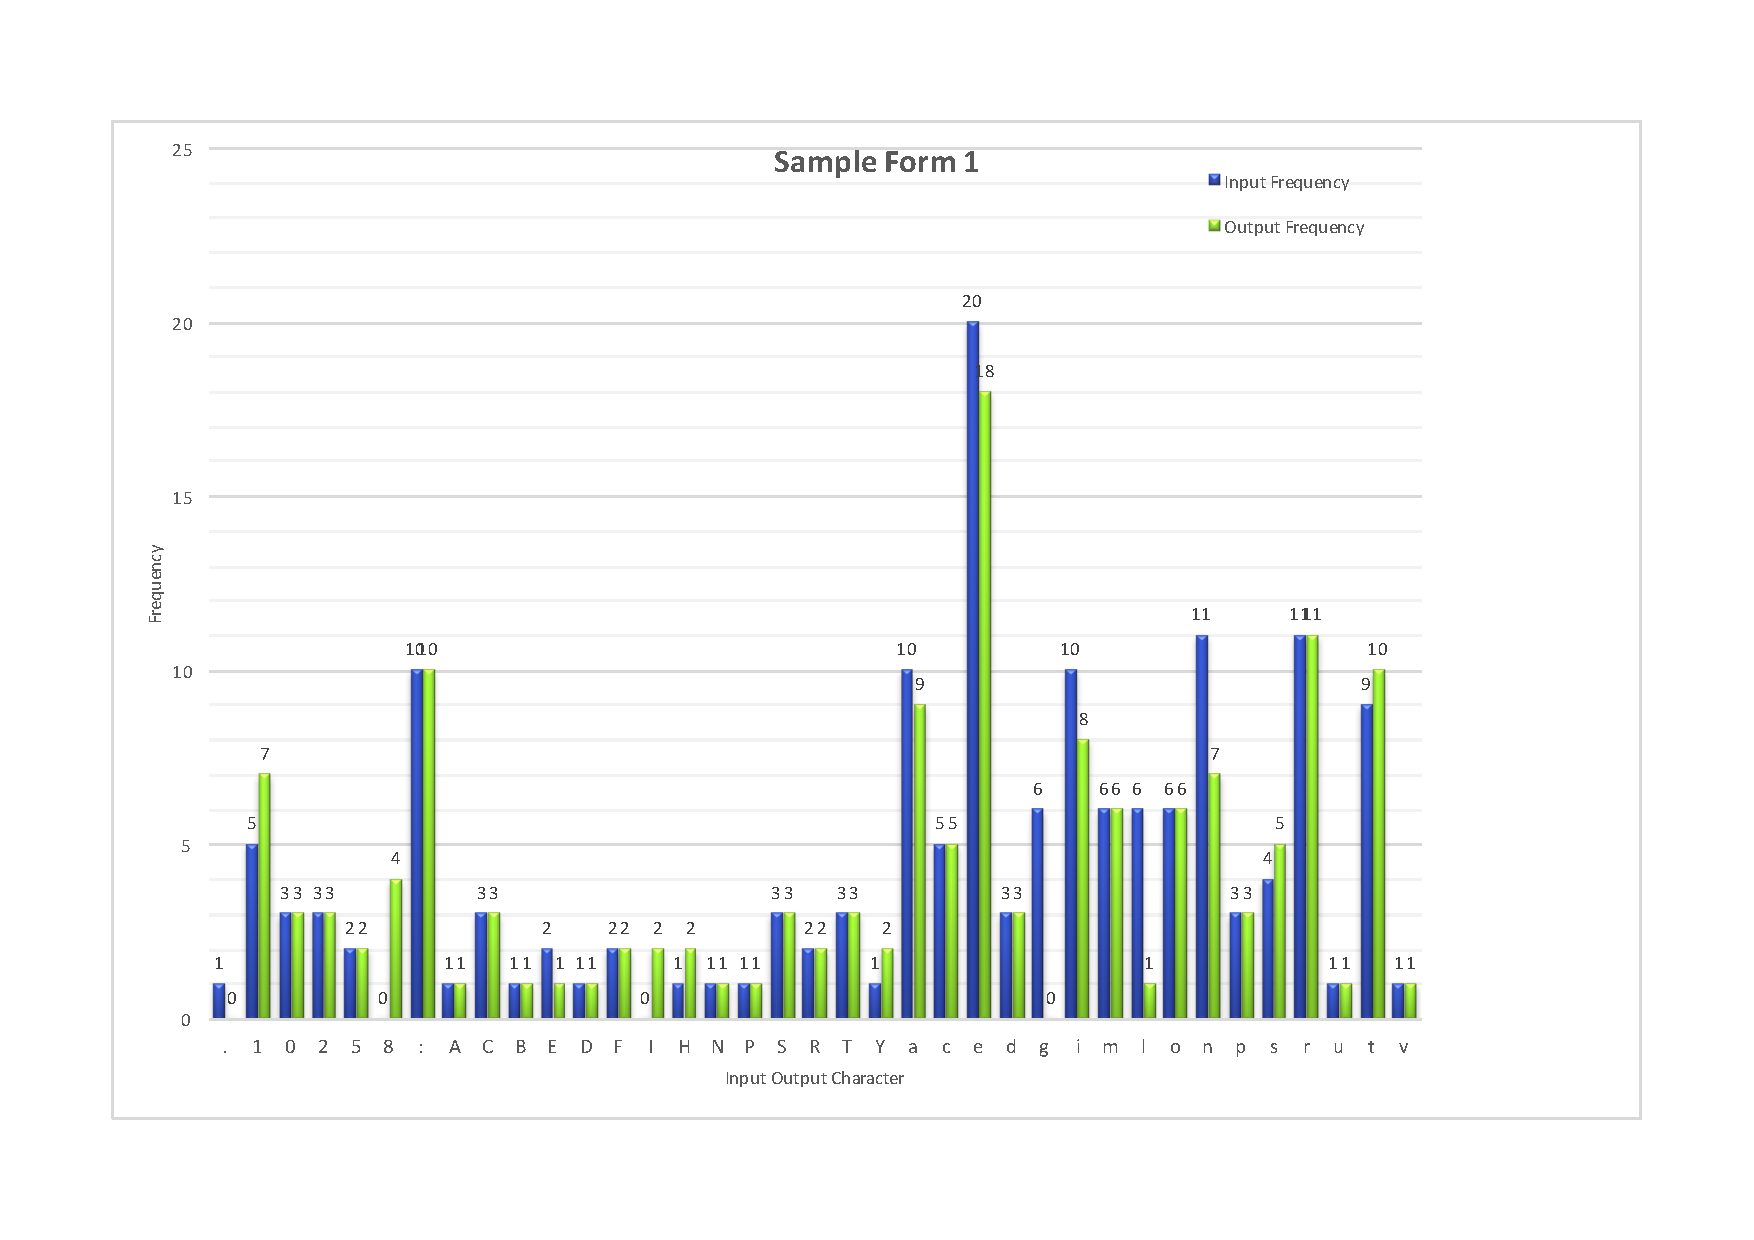
\includegraphics[width=1\textwidth]{form1.pdf}
\caption {Bar chart Input Output Frequency of English Sample form 1}
\label {fig:bar1}
\end{figure}
According to the table \ref{tab:Table1} \& bar chart \ref{fig:bar1} we can say that, input and output frequency of sample English form-01 for the characters 0, 2, 5 ,: ,A ,B ,C ,D ,F ,I ,N ,P ,R ,S ,T ,Y ,a ,c ,d ,l ,o ,p ,r ,s ,t ,u ,v are perfect. But for the 1, 8, E, H, i, characters output frequencies are not perfect. 
\subsection{Sample form 2}

\begin{figure}[H]
\centering
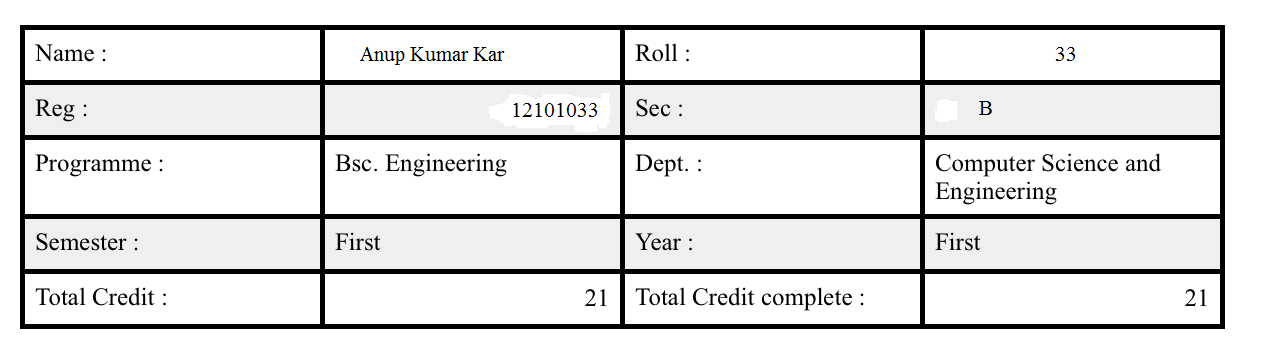
\includegraphics[width=1\textwidth]{form2.png}
\caption {Sample English form 2}
\label {fig:form2}
\end{figure}

\begin{table}[H]
\centering
\begin{tabular}{|p{2cm}|p{2cm}|p{2cm}|}
\hline
character & Input Frequency & Output Frequency \\
\hline
. & 1 & 0\\
\hline
1 & 5 & 7\\
\hline
0 & 2 & 1\\
\hline
3 & 4 & 4\\
\hline
2 & 3 & 3\\
\hline
8 & 0 & 4\\
\hline
: & 10 & 10\\
\hline
A & 1 & 1\\
\hline
C & 3 & 3\\
\hline
B & 2 & 2\\
\hline
E & 2 & 1\\
\hline
D & 1 & 1\\
\hline
F & 2 & 2\\
\hline
I & 0 & 4\\
\hline
H & 0 & 1\\
\hline
K & 2 & 2\\
\hline
O & 0 & 1\\
\hline
N & 1 & 1\\
\hline
P & 1 & 1\\
\hline
S & 3 & 3\\
\hline
R & 2 & 2\\
\hline
T & 2 & 2\\
\hline
Y & 1 & 2\\
\hline
a & 9 & 8\\
\hline
c & 5 & 5\\
\hline
e & 20 & 18\\
\hline
d & 3 & 3\\
\hline
g & 6 & 0\\
\hline
i & 9 & 7\\
\hline
m & 7 & 7\\
\hline
l & 6 & 1\\
\hline
o & 6 & 6\\
\hline
n & 10 & 6\\
\hline
p & 4 & 4\\
\hline
s & 3 & 4\\
\hline
r & 12 & 10\\
\hline
u & 3 & 3\\
\hline
t & 9 & 10\\
\hline
\end{tabular}
\caption {Comparison between Input and Output frequency of Sample Input 2}
\label {tab:Table2}
\end{table}

\begin{figure}[H]
\centering
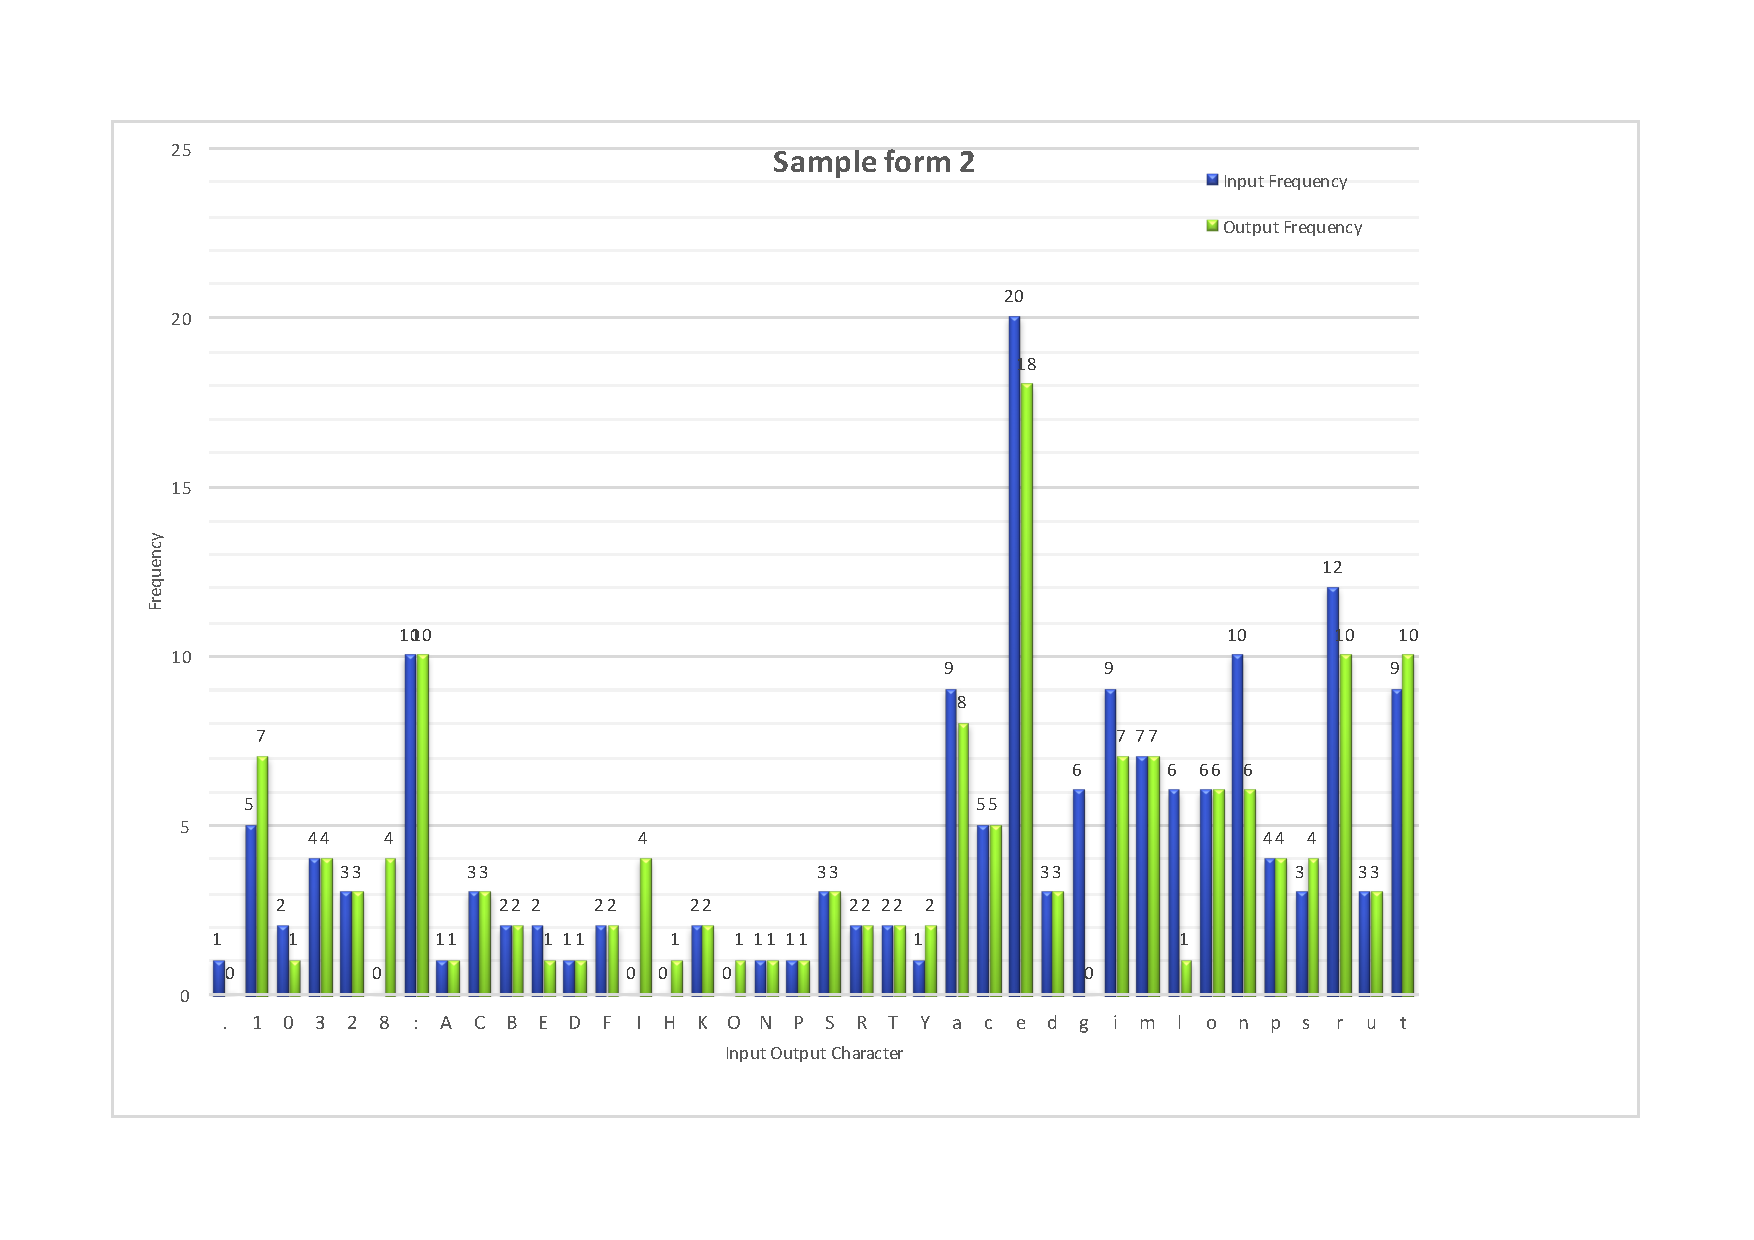
\includegraphics[width=1\textwidth]{form2.pdf}
\caption {Bar chart Input Output Frequency of Sample form 2}
\label {fig:bar2}
\end{figure}
According to the table \ref{tab:Table2} \& bar chart \ref{fig:bar2} we can say that, For sample English form-02 the input and output frequencies are perfect for the characters 2, 3 , :  , A , B, C, D, F, K, N, P, R, T, e, m, u. For the characters 0, 1, 8, E, H, I, O, S, Y, a, c, i, n, o , p, r, s, t outputs are quite different. 
\subsection{Sample form 3}

\begin{figure}[H]
\centering
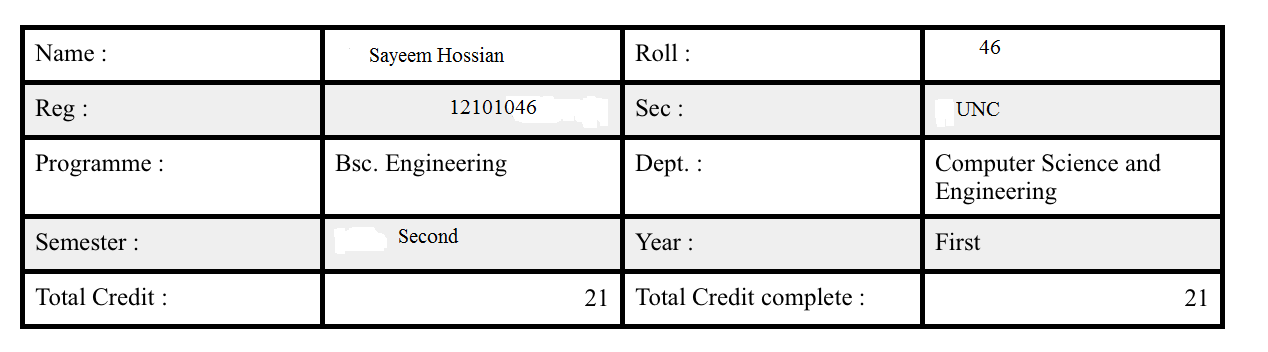
\includegraphics[width=1\textwidth]{form3.png}
\caption {Sample English form 3}
\label {fig:form3}
\end{figure}

\begin{table}[H]
\centering
\begin{tabular}{|p{2cm}|p{2cm}|p{2cm}|}
\hline
character & Input Frequency & Output Frequency \\
\hline
. & 1 & 0\\
\hline
1 & 5 & 7\\
\hline
0 & 2 & 1\\
\hline
2 & 3 & 3\\
\hline
4 & 2 & 2\\
\hline
6 & 2 & 2\\
\hline
8 & 0 & 4\\
\hline
: & 10 & 10\\
\hline
C & 4 & 4\\
\hline
B & 1 & 1\\
\hline
E & 2 & 1\\
\hline
D & 1 & 1\\
\hline
F & 1 & 1\\
\hline
I & 0 & 2\\
\hline
H & 1 & 2\\
\hline
O & 0 & 1\\
\hline
N & 2 & 2\\
\hline
P & 1 & 1\\
\hline
S & 5 & 5\\
\hline
R & 2 & 2\\
\hline
U & 1 & 1\\
\hline
T & 2 & 2\\
\hline
V & 0 & 2\\
\hline
Y & 1 & 2\\
\hline
a & 9 & 8\\
\hline
c & 6 & 6\\
\hline
e & 23 & 21\\
\hline
d & 4 & 4\\
\hline
g & 6 & 0\\
\hline
i & 9 & 7\\
\hline
m & 7 & 7\\
\hline
l & 6 & 1\\
\hline
o & 8 & 8\\
\hline
n & 11 & 7\\
\hline
p & 3 & 3\\
\hline
s & 4 & 5\\
\hline
r & 9 & 9\\
\hline
u & 1 & 1\\
\hline
t & 8 & 9\\
\hline
y & 1 & 1\\
\hline
\end{tabular}
\caption {Comparison between Input and Output frequency of Sample Input 3}
\label {tab:Table3}
\end{table}

\begin{figure}[H]
\centering
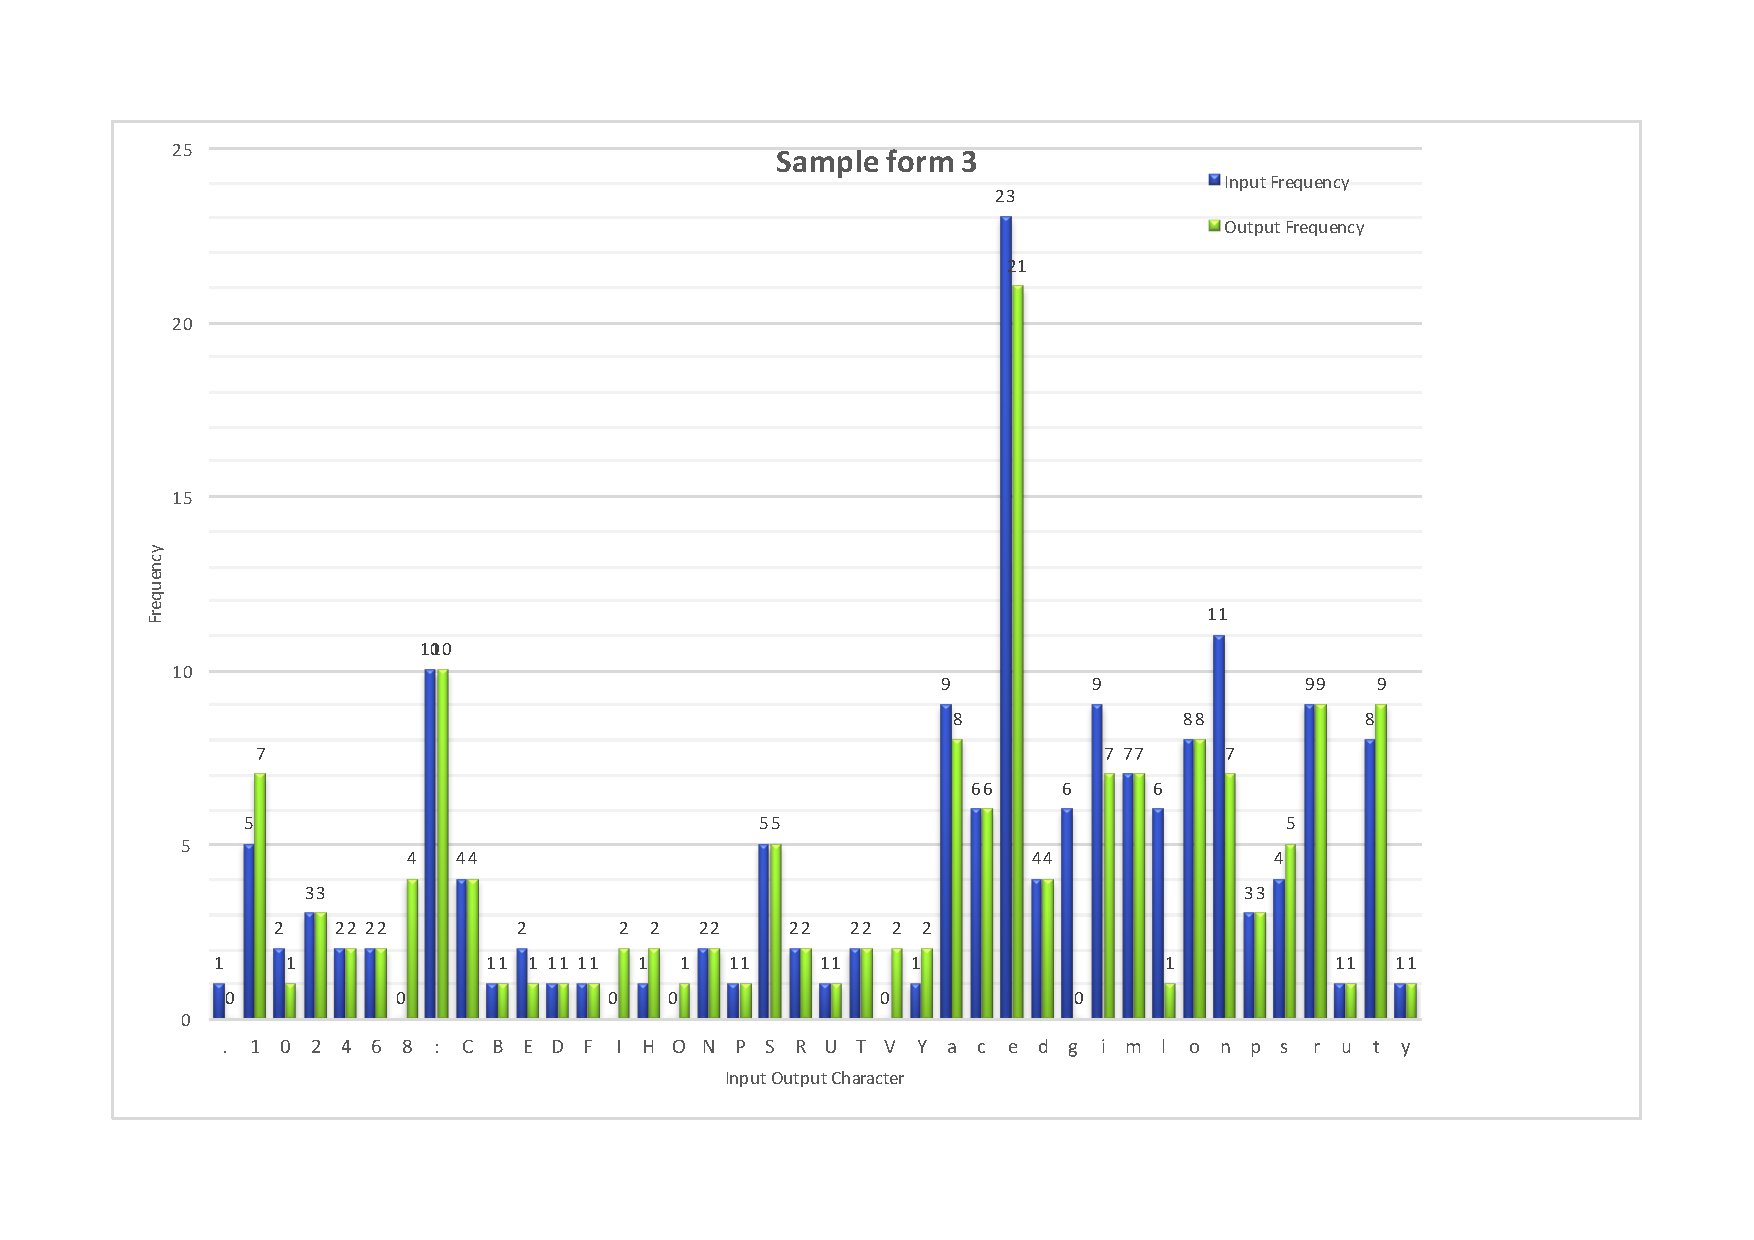
\includegraphics[width=1\textwidth]{form3.pdf}
\caption {Bar chart Input Output Frequency of Sample form 3}
\label {fig:bar3}
\end{figure}
According to the table \ref{tab:Table3} \& bar chart \ref{fig:bar3} we can say that, for sample English form-3 the input and output frequencies are perfect for the characters 2, 4, 6, :, B, C, D, F, N, P, R, S, T, U, c, d, e, m, n, o, p, r, s, t, u, y for sample English form-03. For the characters 0, 1, 8, E, H, I, O, V, Y, a, i and l input and output frequencies are not equal. 

\subsection{Sample form 4}

\begin{figure}[H]
\centering
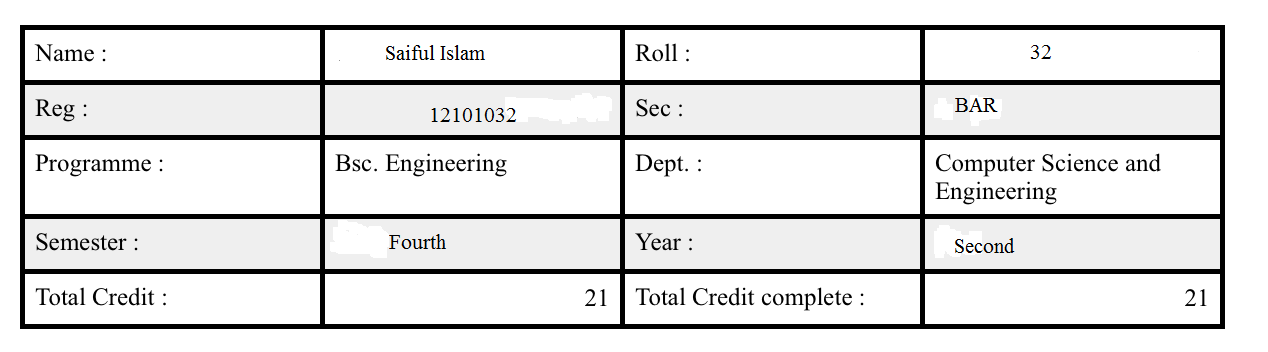
\includegraphics[width=1\textwidth]{form4.png}
\caption {Sample English form 4}
\label {fig:form4}
\end{figure}

\begin{table}[H]
\centering
\begin{tabular}{|p{2cm}|p{2cm}|p{2cm}|}
\hline
character & Input Frequency & Output Frequency \\
\hline
. & 1 & 0\\
\hline
1 & 5 & 10\\
\hline
0 & 2 & 0\\
\hline
3 & 2 & 2\\
\hline
2 & 5 & 5\\
\hline
8 & 0 & 4\\
\hline
: & 10 & 10\\
\hline
A & 1 & 1\\
\hline
C & 3 & 3\\
\hline
B & 2 & 2\\
\hline
E & 2 & 1\\
\hline
D & 1 & 1\\
\hline
F & 1 & 1\\
\hline
I & 1 & 2\\
\hline
H & 0 & 1\\
\hline
O & 0 & 2\\
\hline
N & 1 & 1\\
\hline
P & 1 & 1\\
\hline
S & 5 & 5\\
\hline
R & 3 & 3\\
\hline
T & 2 & 2\\
\hline
Y & 1 & 2\\
\hline
a & 8 & 8\\
\hline
c & 6 & 6\\
\hline
b & 0 & 1\\
\hline
e & 21 & 19\\
\hline
d & 4 & 4\\
\hline
g & 6 & 0\\
\hline
f & 1 & 1\\
\hline
i & 8 & 6\\
\hline
h & 1 & 0\\
\hline
m & 7 & 7\\
\hline
l & 7 & 1\\
\hline
o & 8 & 8\\
\hline
n & 9 & 6\\
\hline
p & 3 & 3\\
\hline
s & 3 & 3\\
\hline
r & 10 & 8\\
\hline
u & 3 & 3\\
\hline
t & 9 & 10\\
\hline
\end{tabular}
\caption {Comparison between Input and Output frequency of Sample Input 4}
\label {tab:Table4}
\end{table}

\begin{figure}[H]
\centering
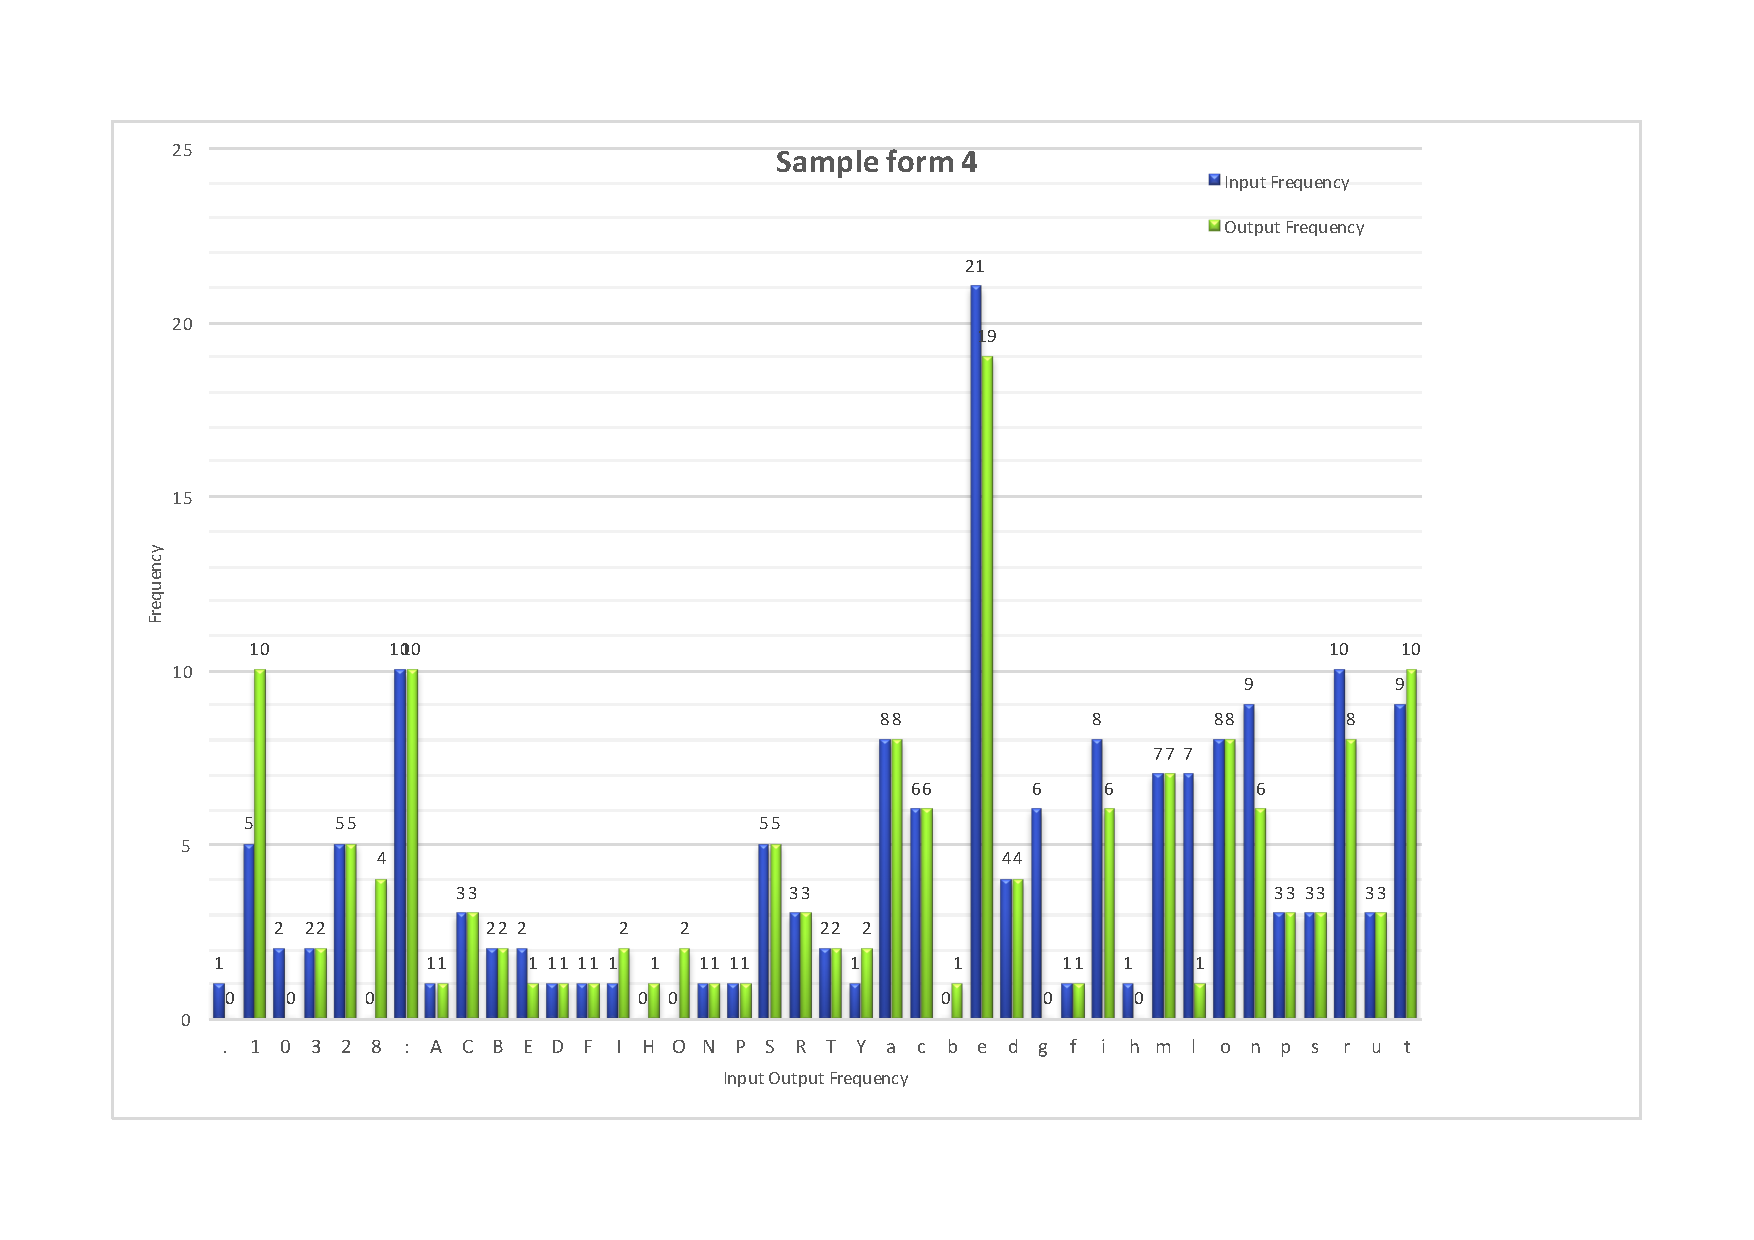
\includegraphics[width=1\textwidth]{form4.pdf}
\caption {Bar chart Input Output Frequency of Sample form 4}
\label {fig:bar4}
\end{figure}

According to the table \ref{tab:Table4} \& bar chart \ref{fig:bar4} we can say that, for sample English form-4 the input and output frequencies are perfect for the characters 2, 3, :, A, C, D, E, F, H, I, N, O, P, R, S, T, Y, a, b, d, f, i, l, m, n, r, s, u for sample English form-03. For the characters ., 0, 1, 8, E, H, I, O, V, Y, a, b, h, n, i, r, t and l input and output frequencies are not equal. 

\subsection{Sample form 5}

\begin{figure}[H]
\centering
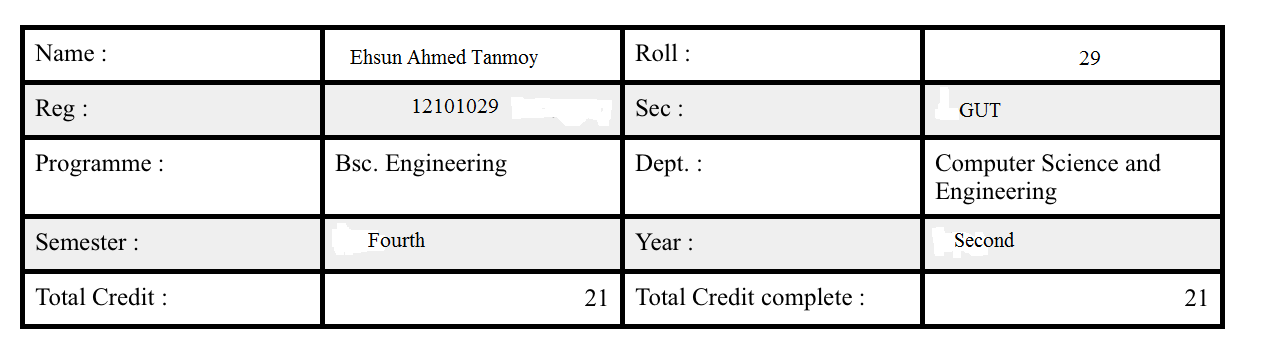
\includegraphics[width=1\textwidth]{form5.png}
\caption {Sample English form 5}
\label {fig:form4}
\end{figure}

\begin{table}[H]
\centering
\begin{tabular}{|p{2cm}|p{2cm}|p{2cm}|}
\hline
character & Input Frequency & Output Frequency \\
\hline
. & 1 & 0\\
\hline
1 & 5 & 7\\
\hline
0 & 2 & 0\\
\hline
2 & 5 & 5\\
\hline
9 & 2 & 2\\
\hline
8 & 0 & 4\\
\hline
: & 10 & 10\\
\hline
A & 1 & 1\\
\hline
C & 3 & 3\\
\hline
B & 1 & 1\\
\hline
E & 3 & 2\\
\hline
D & 1 & 1\\
\hline
G & 1 & 1\\
\hline
F & 1 & 1\\
\hline
I & 0 & 2\\
\hline
H & 0 & 1\\
\hline
L & 0 & 1\\
\hline
O & 0 & 2\\
\hline
N & 1 & 1\\
\hline
P & 1 & 1\\
\hline
S & 4 & 4\\
\hline
R & 2 & 2\\
\hline
U & 1 & 1\\
\hline
T & 4 & 4\\
\hline
Y & 1 & 2\\
\hline
a & 7 & 7\\
\hline
c & 6 & 6\\
\hline
b & 0 & 1\\
\hline
e & 22 & 20\\
\hline
d & 5 & 5\\
\hline
g & 6 & 0\\
\hline
i & 8 & 5\\
\hline
h & 2 & 2\\
\hline
m & 8 & 9\\
\hline
l & 5 & 1\\
\hline
o & 8 & 9\\
\hline
n & 11 & 8\\
\hline
p & 3 & 3\\
\hline
s & 4 & 3\\
\hline
r & 10 & 8\\
\hline
u & 2 & 2\\
\hline
t & 9 & 8\\
\hline
y & 1 & 1\\
\hline
\end{tabular}
\caption {Comparison between Input and Output frequency of Sample Input 5}
\label {tab:Table5}
\end{table}

\begin{figure}[H]
\centering
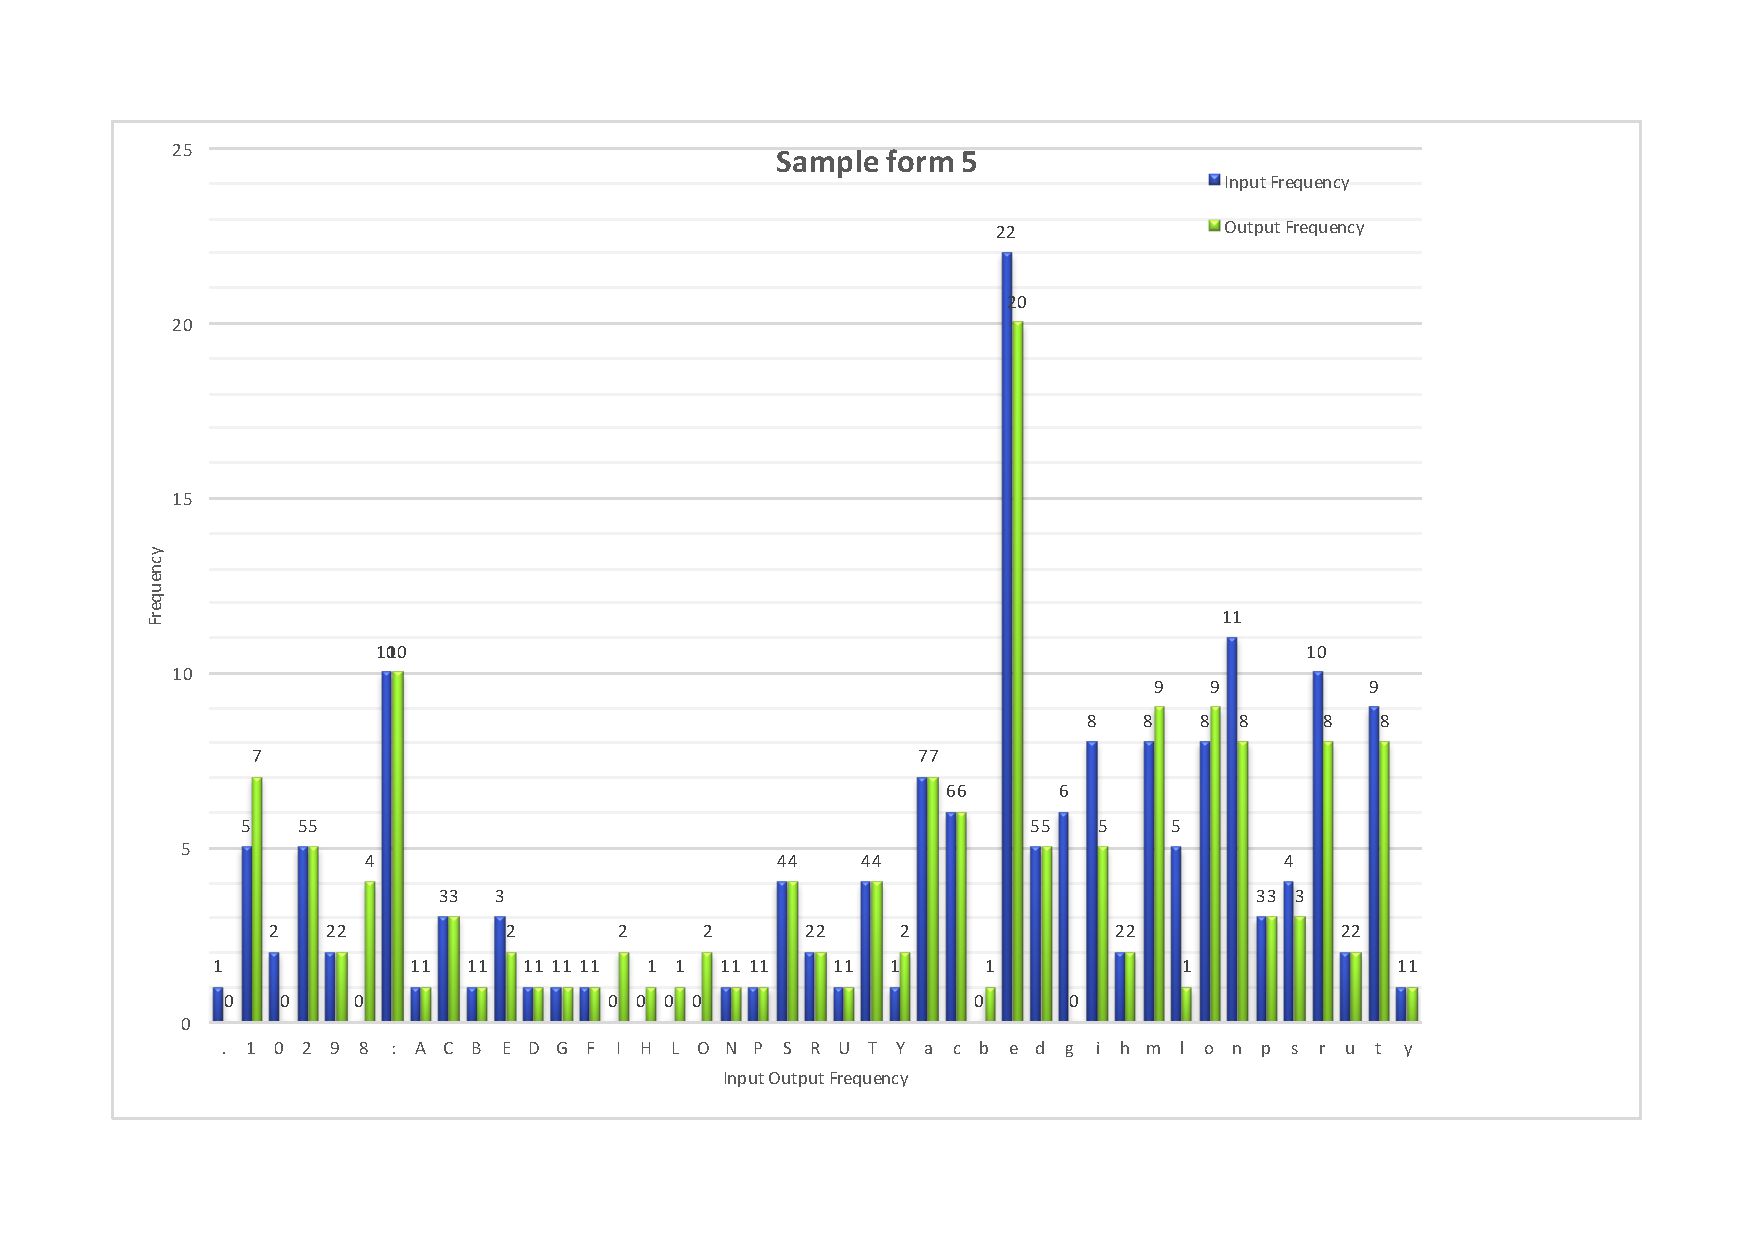
\includegraphics[width=1\textwidth]{form5.pdf}
\caption {Bar chart Input Output Frequency of Sample form 4}
\label {fig:bar5}
\end{figure}

According to these frequency table and bar chart we can say our tarined tesseract accuracy is upto 85\%. Here accuracy of character 'g' is below average. Most of the time character 'g' recognize as digit '8'. And double 'l' character (Ex: Roll) recognize as 'H'. It can be resolve with more frequent fonts training.

\section{Performance for Bangla form}
The result of Bangla form depends on the tesseract training data same as English form. For Bangla we train "Siyam rupali" font. Here we show our some output result and analysis of our training data.
\subsection{Sample form 1}
\begin{figure}[H]
\centering
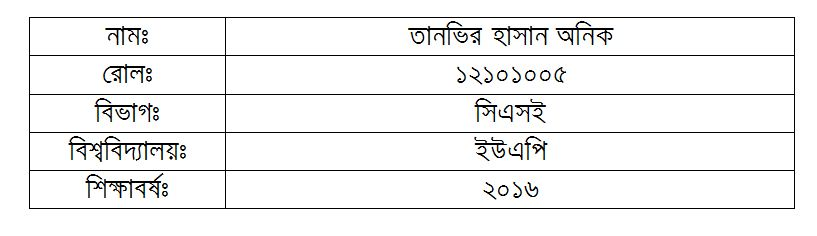
\includegraphics[width=1\textwidth]{formBen01.JPG}
\caption {Sample Bangla form 1}
\label {fig:FormBan1}
\end{figure}

\begin{table}[H]
\centering
\begin{tabular}{|p{2cm}|p{2cm}|p{2cm}|}
\hline
character & Input Frequency & Output Frequency \\
\hline
{\bengalifont ঃ} & 3 & 5\\
\hline
{\bengalifont অ} & 1 & 1\\
\hline
{\bengalifont ই} & 1 & 2\\
\hline
{\bengalifont উ} & 1 & 1\\
\hline
{\bengalifont এ} & 2 & 2\\
\hline
{\bengalifont ক} & 2 & 2\\
\hline
{\bengalifont গ} & 1 & 1\\
\hline
{\bengalifont চ} & 1 & 0\\
\hline
{\bengalifont ত} & 1 & 1\\
\hline
{\bengalifont '} & 8 & 0\\
\hline
{\bengalifont র} & 2 & 3\\
\hline
{\bengalifont ন} & 4 & 4\\
\hline
{\bengalifont প} & 1 & 1\\
\hline
{\bengalifont ভ} & 2 & 2\\
\hline
{\bengalifont ব} & 6 & 5\\
\hline
{\bengalifont য} & 2 & 1\\
\hline
{\bengalifont ম} & 1 & 1\\
\hline
{\bengalifont 0} & 4 & 0\\
\hline
{\bengalifont ল} & 4 & 2\\
\hline
{\bengalifont ষ} & 2 & 2\\
\hline
{\bengalifont শ} & 2 & 2\\
\hline
{\bengalifont হ} & 1 & 1\\
\hline
{\bengalifont স} & 1 & 3\\
\hline
{\bengalifont ;} & 1 & 0\\
\hline
{\bengalifont ়} & 1 & 0\\
\hline
{\bengalifont ি} & 8 & 7\\
\hline
{\bengalifont া} & 7 & 7\\
\hline
{\bengalifont ী} & 0 & 1\\
\hline
{\bengalifont ো} & 1 & 1\\
\hline
{\bengalifont ্} & 6 & 4\\
\hline
{\bengalifont য়} & 0 & 1\\
\hline
{\bengalifont ১} & 4 & 4\\
\hline
{\bengalifont ০} & 0 & 4\\
\hline
{\bengalifont ২} & 2 & 2\\
\hline
{\bengalifont ৫} & 1 & 1\\
\hline
{\bengalifont দ} & 1 & 1\\
\hline
{\bengalifont ৬} & 1 & 1\\
\hline
\end{tabular}
\caption { Comparison between Input and Output frequency of Sample Input 1}
\label {tab:BTable1}
\end{table}

\begin{figure}[H]
\centering
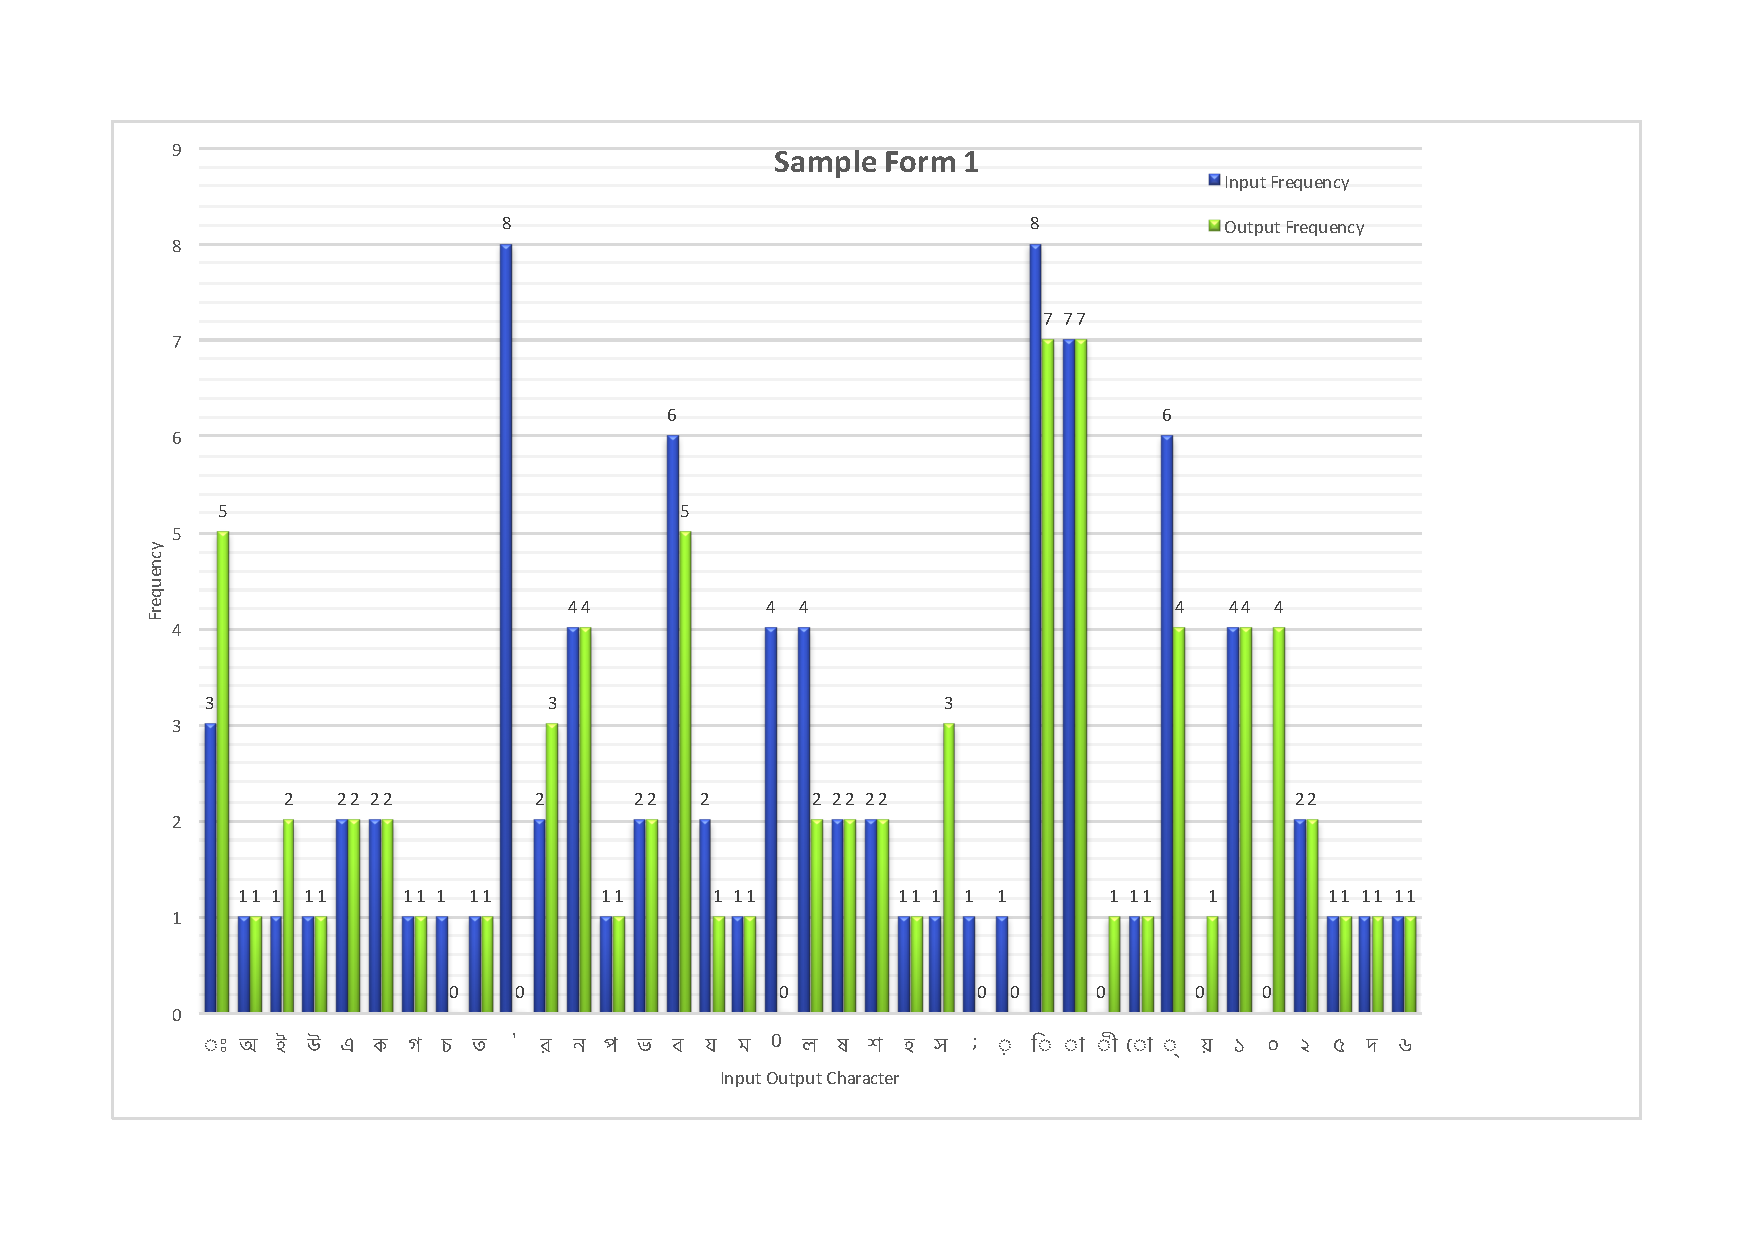
\includegraphics[width=1\textwidth]{Bform1.pdf}
\caption {Bar chart Input Output Frequency of Sample form 1}
\label {fig:Bbar1}
\end{figure}




\subsection{Sample form 2}
\begin{figure}[H]
\centering
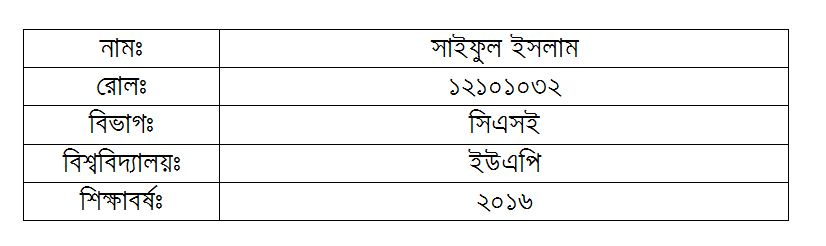
\includegraphics[width=1\textwidth]{formBen02.JPG}
\caption {Sample Bangla form 2}
\label {fig:FormBan2}
\end{figure}

\begin{table}[H]
\centering
\begin{tabular}{|p{2cm}|p{2cm}|p{2cm}|}
\hline
character & Input Frequency & Output Frequency \\
\hline
{\bengalifont ঃ} & 4 & 5\\
\hline
{\bengalifont ই} & 4 & 4\\
\hline
{\bengalifont উ} & 0 & 1\\
\hline
{\bengalifont ঊ} & 1 & 0\\
\hline
{\bengalifont এ} & 2 & 2\\
\hline
{\bengalifont ক} & 1 & 1\\
\hline
{\bengalifont গ} & 1 & 1\\
\hline
{\bengalifont ’} & 1 & 0\\
\hline
{\bengalifont চ} & 1 & 0\\
\hline
{\bengalifont '} & 7 & 0\\
\hline
{\bengalifont দ} & 1 & 1\\
\hline
{\bengalifont ন} & 1 & 1\\
\hline
{\bengalifont ফ} & 1 & 1\\
\hline
{\bengalifont প} & 1 & 1\\
\hline
{\bengalifont ভ} & 1 & 1\\
\hline
{\bengalifont ব} & 6 & 5\\
\hline
{\bengalifont য} & 2 & 1\\
\hline
{\bengalifont ম} & 2 & 2\\
\hline
{\bengalifont র} & 1 & 2\\
\hline
{\bengalifont ল} & 5 & 4\\
\hline
{\bengalifont ষ} & 2 & 2\\
\hline
{\bengalifont শ} & 2 & 2\\
\hline
{\bengalifont স} & 4 & 4\\
\hline
{\bengalifont ়} & 1 & 0\\
\hline
{\bengalifont ি} & 6 & 6\\
\hline
{\bengalifont া} & 6 & 6\\
\hline
{\bengalifont ু} & 1 & 1\\
\hline
{\bengalifont ে} & 1 & 0\\
\hline
{\bengalifont ো} & 1 & 1\\
\hline
{\bengalifont ্} & 6 & 4\\
\hline
{\bengalifont য়} & 0 & 1\\
\hline
{\bengalifont ১} & 4 & 4\\
\hline
{\bengalifont ০} & 3 & 3\\
\hline
{\bengalifont ৩} & 1 & 1\\
\hline
{\bengalifont ২} & 3 & 3\\
\hline
{\bengalifont ৬} & 1 & 1\\
\hline
\end{tabular}
\caption { Comparison between Input and Output frequency of Sample Input 2}
\label {tab:BTable2}
\end{table}


\begin{figure}[H]
\centering
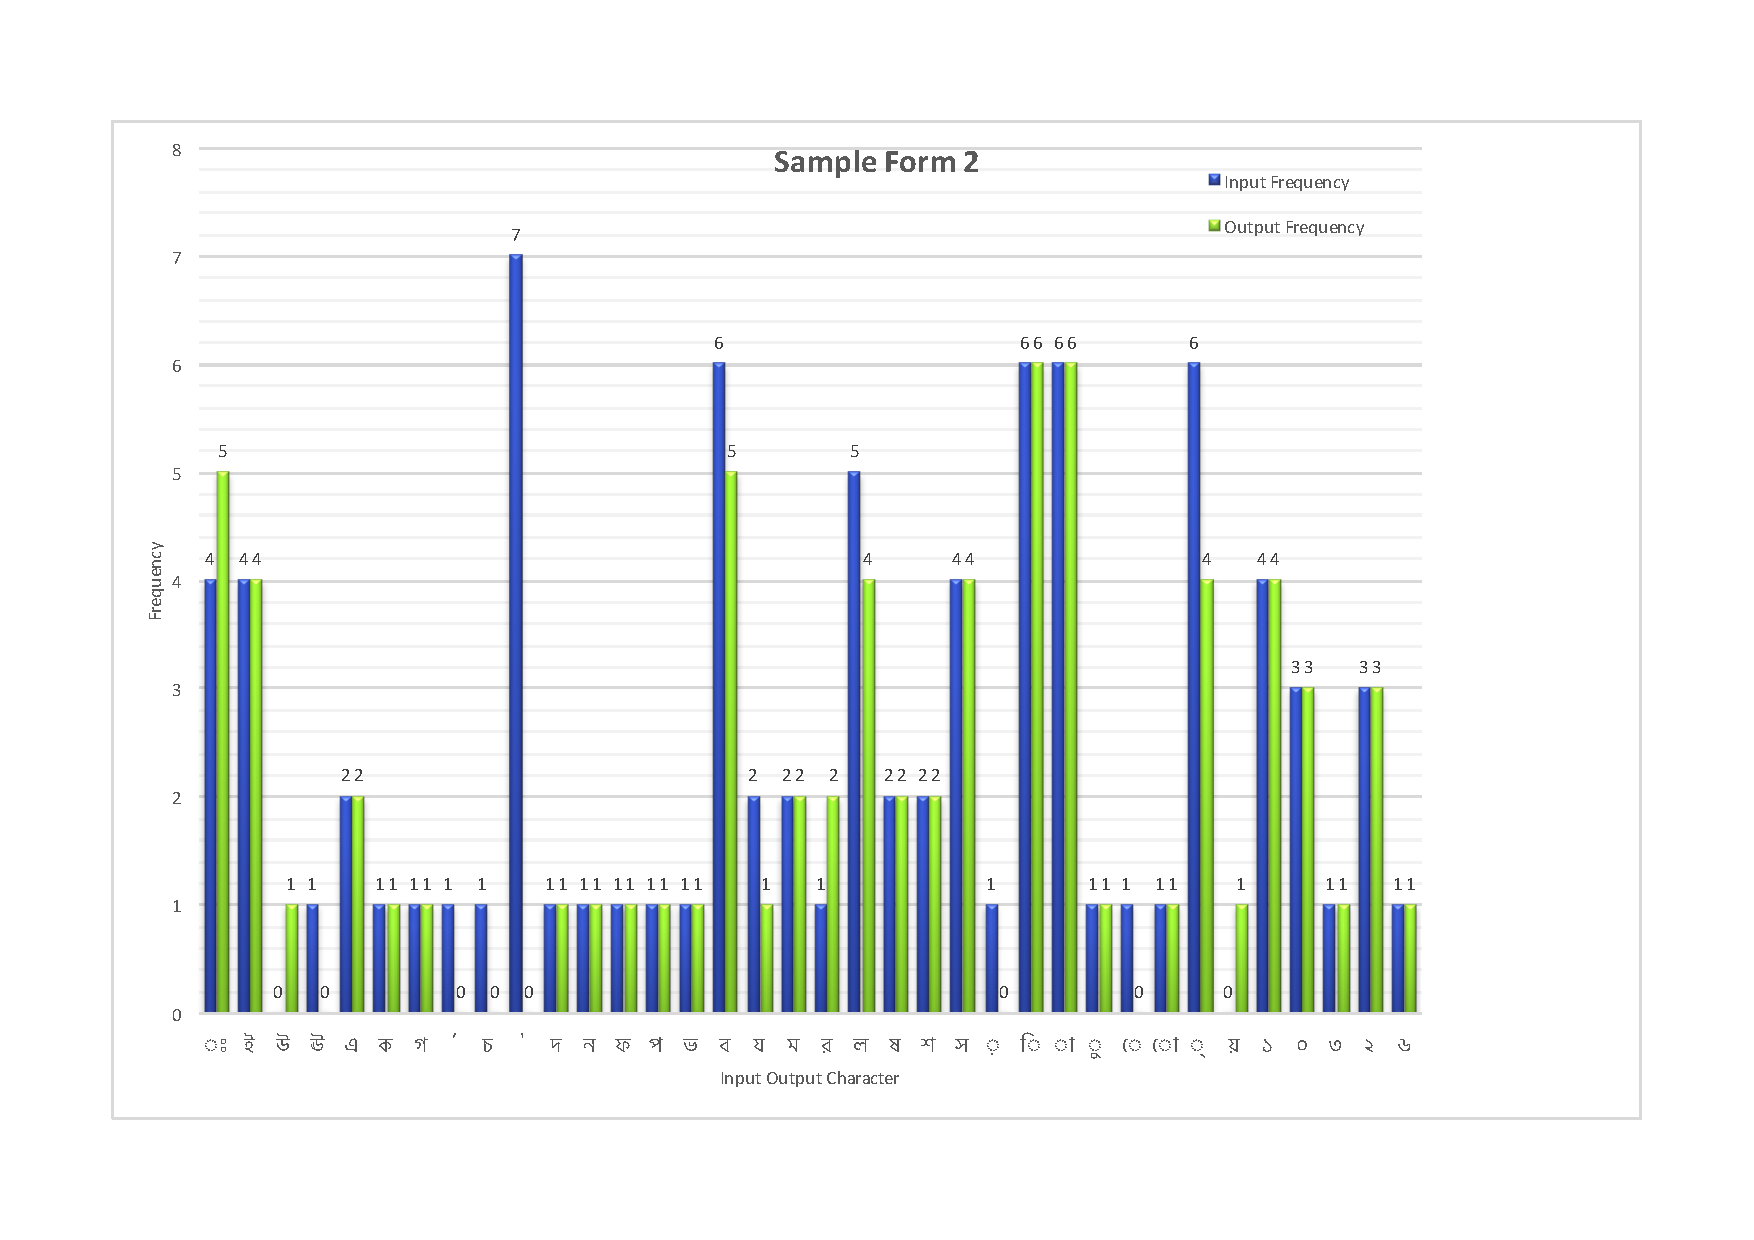
\includegraphics[width=1\textwidth]{Bform2.pdf}
\caption {Bar chart Input Output Frequency of Sample form 2}
\label {fig:Bbar2}
\end{figure}



\subsection{Sample form 3}
\begin{figure}[H]
\centering
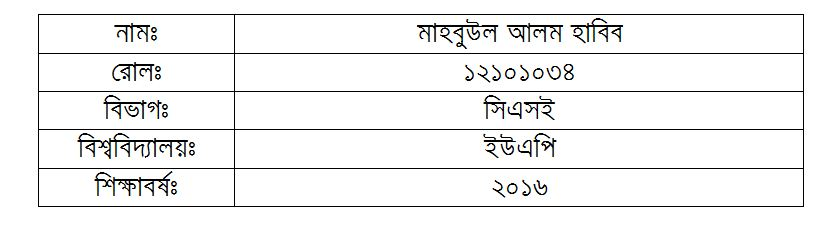
\includegraphics[width=1\textwidth]{formBen03.JPG}
\caption {Sample Bangla form 3}
\label {fig:FormBan3}
\end{figure}


\begin{table}[H]
\centering
\begin{tabular}{|p{2cm}|p{2cm}|p{2cm}|}
\hline
character & Input Frequency & Output Frequency \\
\hline
{\bengalifont ঃ} & 4 & 5\\
\hline
{\bengalifont ই} & 1 & 2\\
\hline
{\bengalifont আ} & 1 & 1\\
\hline
{\bengalifont উ} & 1 & 2\\
\hline
{\bengalifont ঊ} & 1 & 0\\
\hline
{\bengalifont এ} & 2 & 2\\
\hline
{\bengalifont ক} & 1 & 1\\
\hline
{\bengalifont গ} & 1 & 1\\
\hline
{\bengalifont ’} & 1 & 0\\
\hline
{\bengalifont চ} & 1 & 0\\
\hline
{\bengalifont '} & 8 & 0\\
\hline
{\bengalifont দ} & 1 & 1\\
\hline
{\bengalifont ন} & 1 & 1\\
\hline
{\bengalifont প} & 1 & 1\\
\hline
{\bengalifont ভ} & 1 & 1\\
\hline
{\bengalifont ব} & 9 & 8\\
\hline
{\bengalifont য} & 2 & 1\\
\hline
{\bengalifont ম} & 3 & 3\\
\hline
{\bengalifont 0} & 1 & 0\\
\hline
{\bengalifont ল} & 6 & 4\\
\hline
{\bengalifont ষ} & 2 & 2\\
\hline
{\bengalifont শ} & 2 & 2\\
\hline
{\bengalifont হ} & 2 & 2\\
\hline
{\bengalifont 8} & 1 & 0\\
\hline
{\bengalifont ়} & 1 & 0\\
\hline
{\bengalifont ি} & 7 & 7\\
\hline
{\bengalifont া} & 6 & 6\\
\hline
{\bengalifont ু} & 1 & 1\\
\hline
{\bengalifont ো} & 1 & 1\\
\hline
{\bengalifont ্} & 6 & 4\\
\hline
{\bengalifont র} & 1 & 2\\
\hline
{\bengalifont স} & 0 & 2\\
\hline
{\bengalifont য়} & 0 & 1\\
\hline
{\bengalifont ১} & 4 & 4\\
\hline
{\bengalifont ০} & 2 & 3\\
\hline
{\bengalifont ৩} & 1 & 1\\
\hline
{\bengalifont ২} & 2 & 2\\
\hline
{\bengalifont ৪} & 0 & 1\\
\hline
{\bengalifont ৬} & 1 & 1\\
\hline
\end{tabular}
\caption { Comparison between Input and Output frequency of Sample Input 3}
\label {tab:BTable3}
\end{table}

\begin{figure}[H]
\centering
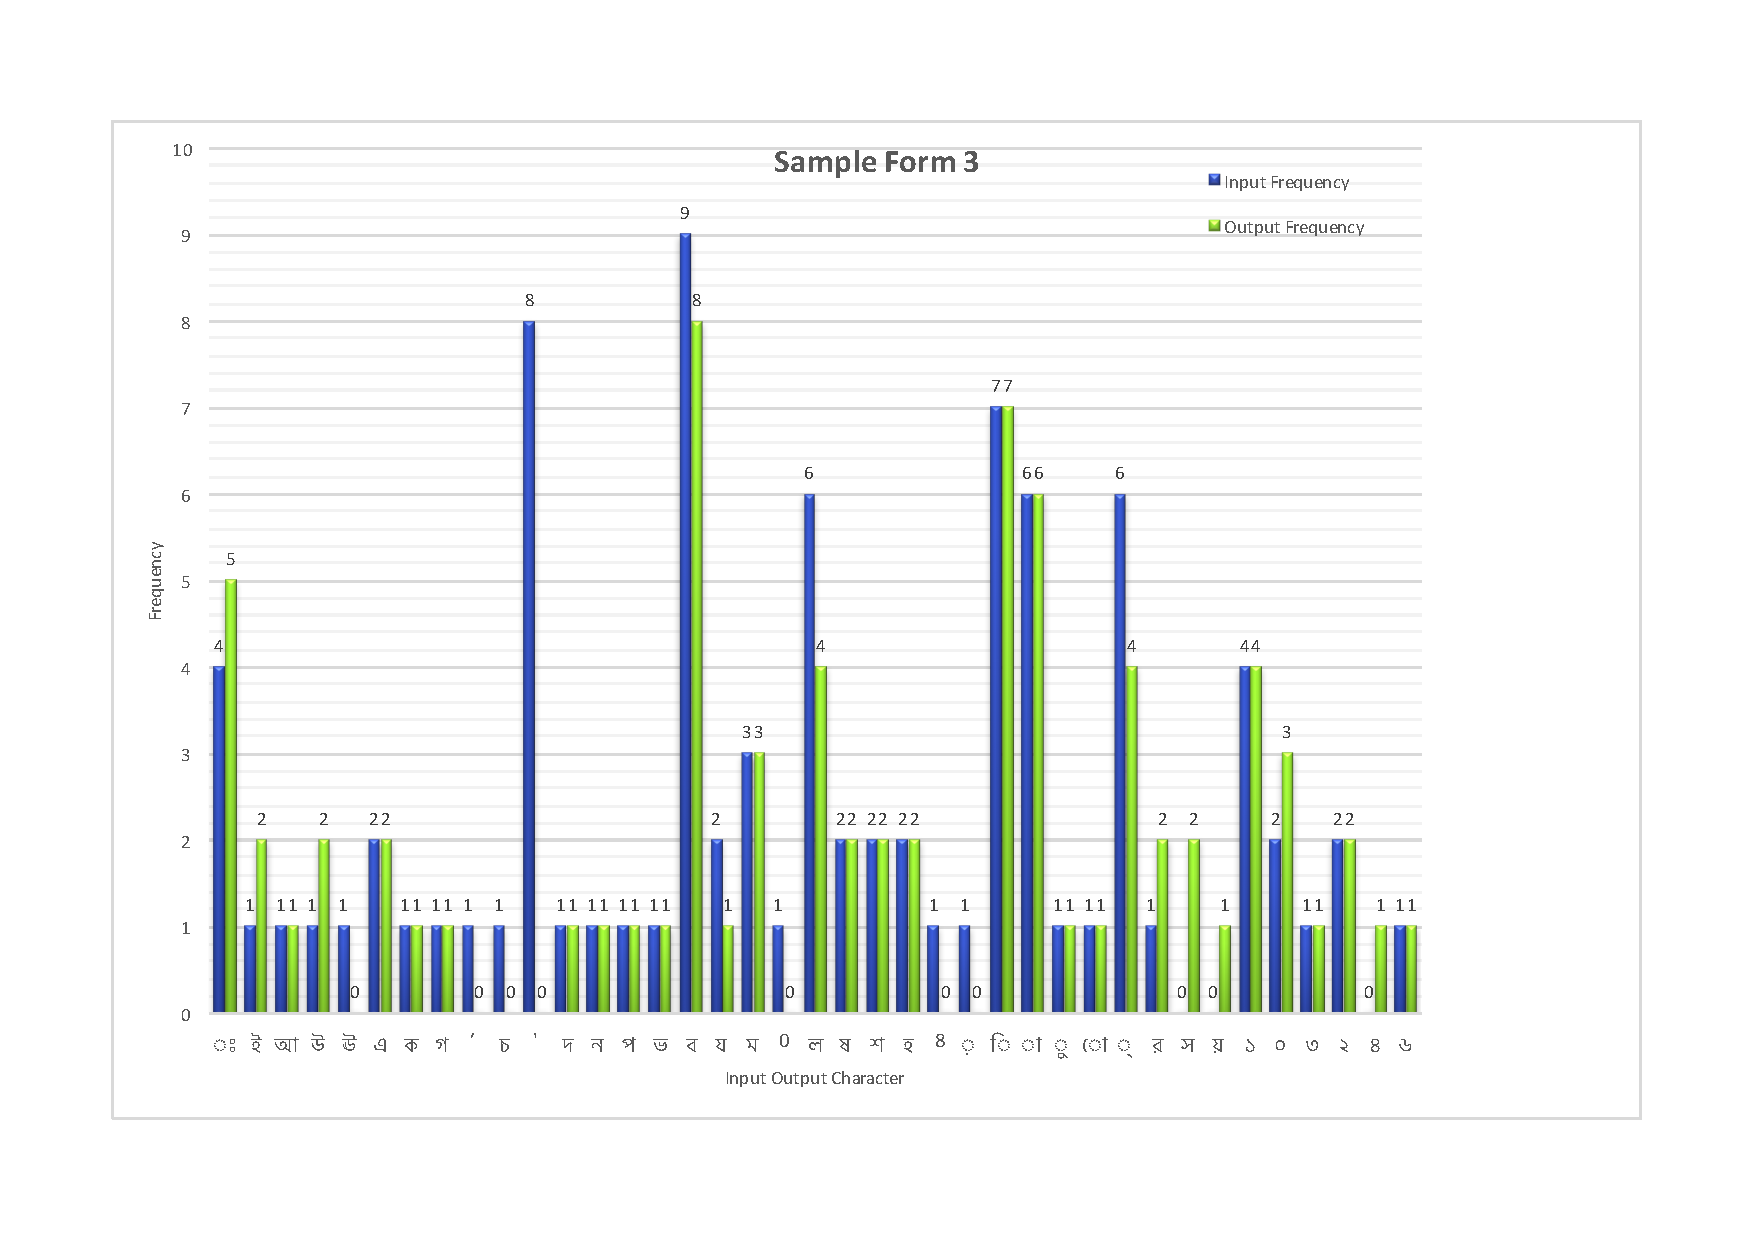
\includegraphics[width=1\textwidth]{Bform3.pdf}
\caption {Bar chart Input Output Frequency of Sample form 3}
\label {fig:Bbar3}
\end{figure}



\subsection{Sample form 4}
\begin{figure}[H]
\centering
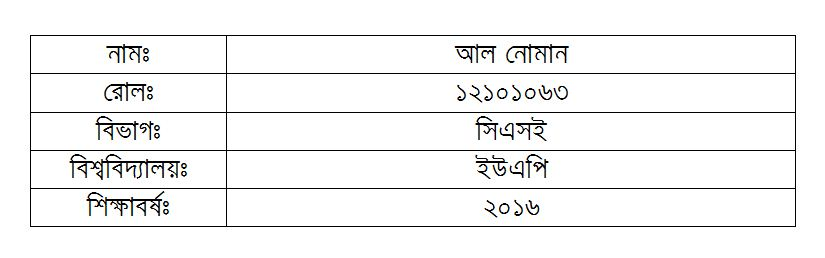
\includegraphics[width=1\textwidth]{formBen04.JPG}
\caption {Sample Bangla form 4}
\label {fig:FormBan4}
\end{figure}

\begin{table}[H]
\centering
\begin{tabular}{|p{2cm}|p{2cm}|p{2cm}|}
\hline
character & Input Frequency & Output Frequency \\
\hline
{\bengalifont ঃ} & 4 & 5\\
\hline
{\bengalifont ই} & 1 & 2\\
\hline
{\bengalifont আ} & 1 & 1\\
\hline
{\bengalifont উ} & 0 & 1\\
\hline
{\bengalifont ঊ} & 1 & 0\\
\hline
{\bengalifont এ} & 2 & 2\\
\hline
{\bengalifont ক} & 1 & 1\\
\hline
{\bengalifont গ} & 1 & 1\\
\hline
{\bengalifont ’} & 1 & 0\\
\hline
{\bengalifont চ} & 1 & 0\\
\hline
{\bengalifont '} & 8 & 0\\
\hline
{\bengalifont দ} & 1 & 1\\
\hline
{\bengalifont ন} & 3 & 3\\
\hline
{\bengalifont প} & 1 & 1\\
\hline
{\bengalifont ভ} & 1 & 1\\
\hline
{\bengalifont ব} & 6 & 5\\
\hline
{\bengalifont য} & 2 & 1\\
\hline
{\bengalifont ম} & 2 & 2\\
\hline
{\bengalifont র} & 1 & 2\\
\hline
{\bengalifont ল} & 5 & 3\\
\hline
{\bengalifont ষ} & 2 & 2\\
\hline
{\bengalifont শ} & 2 & 2\\
\hline
{\bengalifont স} & 0 & 2\\
\hline
{\bengalifont ়} & 1 & 0\\
\hline
{\bengalifont ি} & 6 & 6\\
\hline
{\bengalifont া} & 6 & 5\\
\hline
{\bengalifont ে} & 1 & 0\\
\hline
{\bengalifont ো} & 1 & 2\\
\hline
{\bengalifont ্} & 6 & 4\\
\hline
{\bengalifont য়} & 0 & 1\\
\hline
{\bengalifont ১} & 4 & 4\\
\hline
{\bengalifont ০} & 3 & 3\\
\hline
{\bengalifont ৩} & 1 & 1\\
\hline
{\bengalifont ২} & 2 & 2\\
\hline
{\bengalifont ৬} & 2 & 2\\
\hline
\end{tabular}
\caption { Comparison between Input and Output frequency of Sample Input 4}
\label {tab:BTable4}
\end{table}

\begin{figure}[H]
\centering
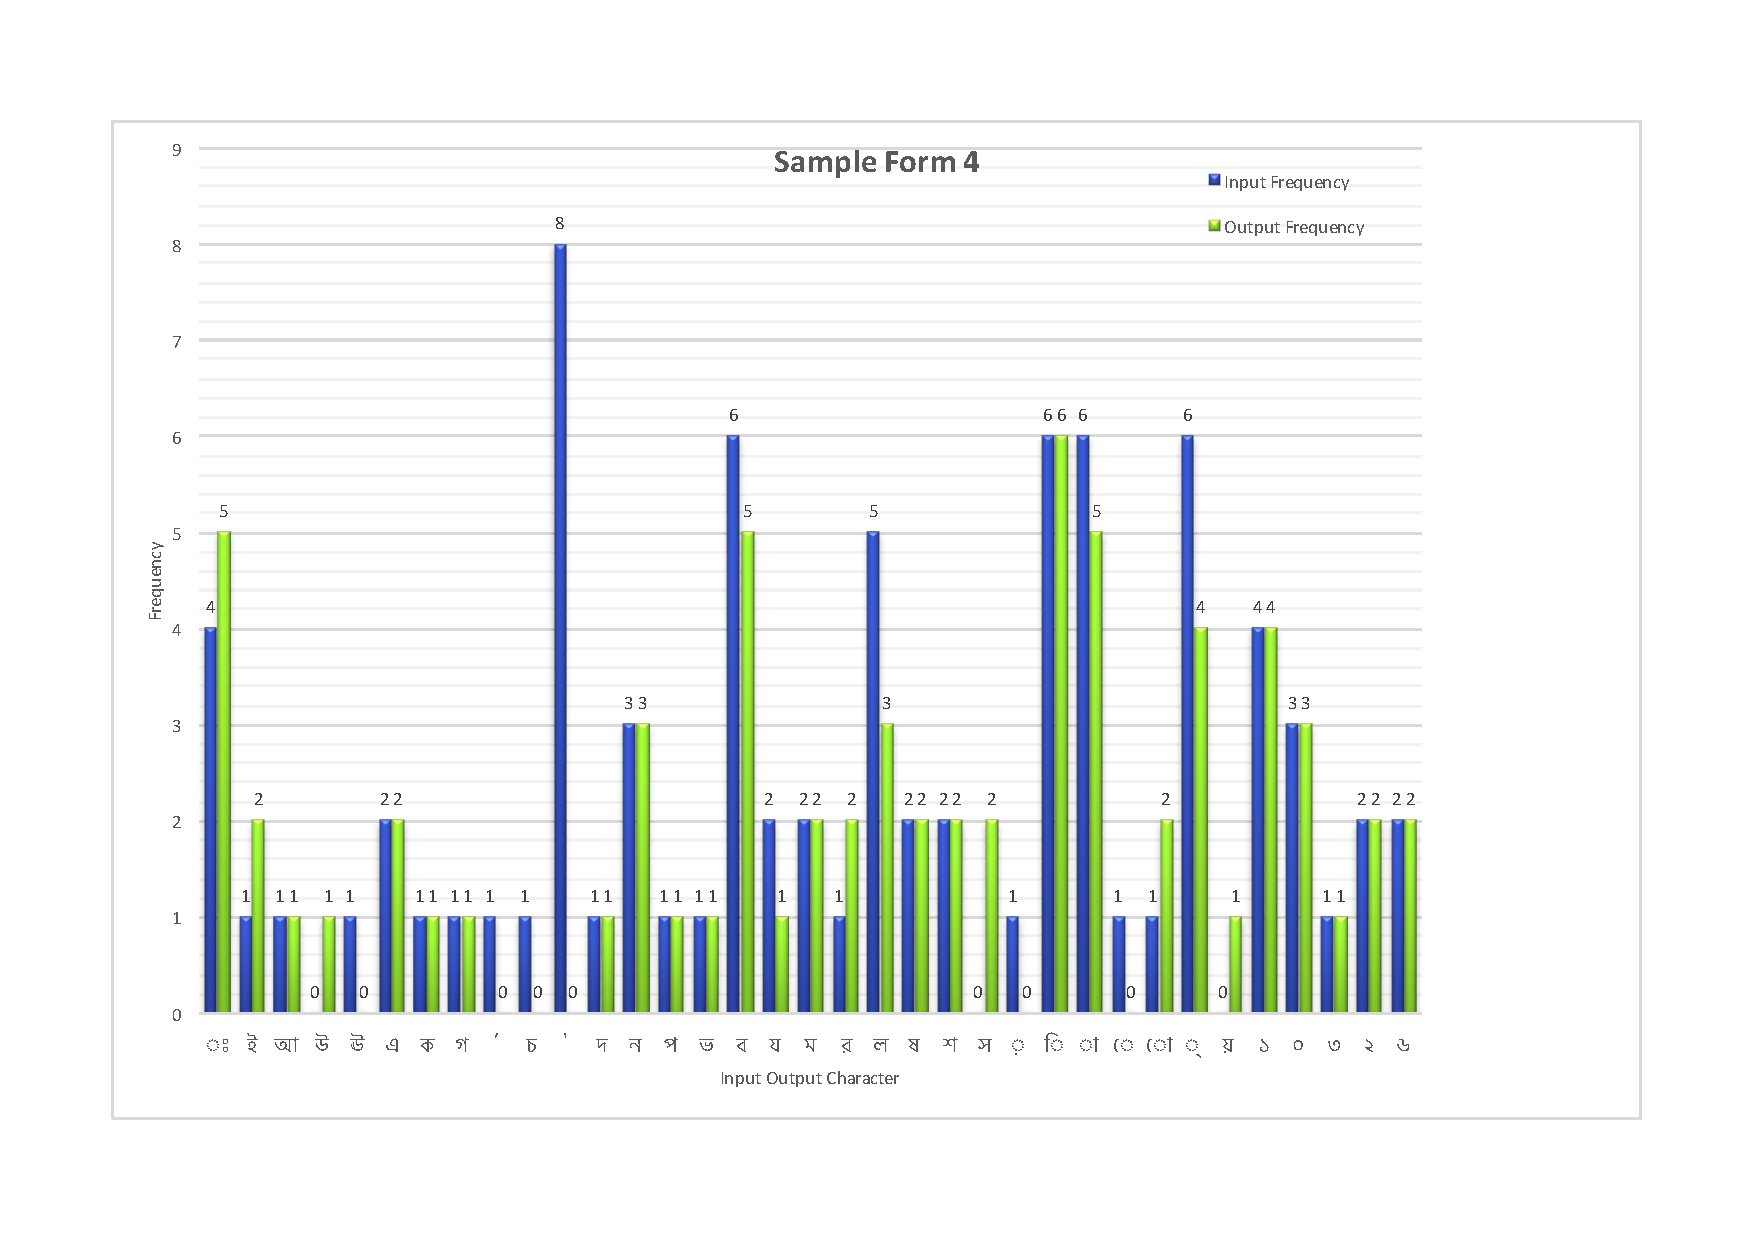
\includegraphics[width=1\textwidth]{Bform4.pdf}
\caption {Bar chart Input Output Frequency of Sample form 4}
\label {fig:Bbar4}
\end{figure}


\subsection{Sample form 5}
\begin{figure}[H]
\centering
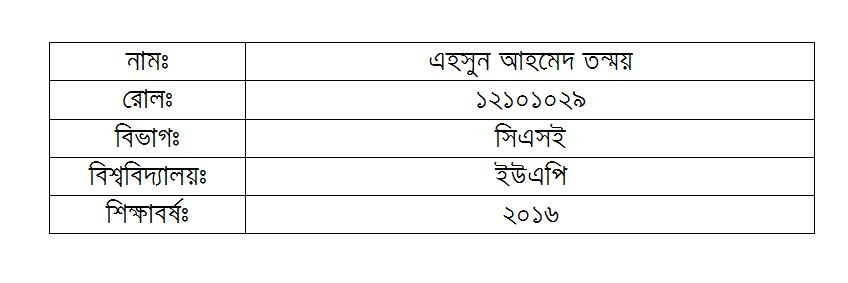
\includegraphics[width=1\textwidth]{formBen05.JPG}
\caption {Sample Bangla form 5}
\label {fig:FormBan5}
\end{figure}

\begin{table}[H]
\centering
\begin{tabular}{|p{2cm}|p{2cm}|p{2cm}|}
\hline
character & Input Frequency & Output Frequency \\
\hline
{\bengalifont ঃ} & 5 & 5\\
\hline
{\bengalifont 0} & 1 & 0\\
\hline
{\bengalifont ই} & 1 & 2\\
\hline
{\bengalifont আ} & 1 & 1\\
\hline
{\bengalifont উ} & 1 & 1\\
\hline
{\bengalifont এ} & 3 & 3\\
\hline
{\bengalifont ক} & 1 & 1\\
\hline
{\bengalifont গ} & 1 & 1\\
\hline
{\bengalifont ’} & 1 & 0\\
\hline
{\bengalifont চ} & 1 & 0\\
\hline
{\bengalifont ত} & 1 & 1\\
\hline
{\bengalifont '} & 7 & 0\\
\hline
{\bengalifont দ} & 2 & 2\\
\hline
{\bengalifont ন} & 4 & 3\\
\hline
{\bengalifont প} & 1 & 1\\
\hline
{\bengalifont ভ} & 1 & 1\\
\hline
{\bengalifont ব} & 6 & 5\\
\hline
{\bengalifont য} & 3 & 1\\
\hline
{\bengalifont ম} & 4 & 3\\
\hline
{\bengalifont র} & 1 & 2\\
\hline
{\bengalifont ল} & 4 & 2\\
\hline
{\bengalifont ষ} & 2 & 2\\
\hline
{\bengalifont শ} & 2 & 2\\
\hline
{\bengalifont হ} & 2 & 2\\
\hline
{\bengalifont স} & 1 & 3\\
\hline
{\bengalifont ়} & 2 & 0\\
\hline
{\bengalifont ি} & 6 & 6\\
\hline
{\bengalifont া} & 5 & 4\\
\hline
{\bengalifont ু} & 1 & 1\\
\hline
{\bengalifont ে} & 1 & 1\\
\hline
{\bengalifont ো} & 1 & 1\\
\hline
{\bengalifont ্} & 7 & 5\\
\hline
{\bengalifont য়} & 0 & 2\\
\hline
{\bengalifont ১} & 4 & 4\\
\hline
{\bengalifont ০} & 2 & 3\\
\hline
{\bengalifont ২} & 3 & 3\\
\hline
{\bengalifont ৬} & 1 & 1\\
\hline
{\bengalifont ৯} & 1 & 1\\
\hline
\end{tabular}
\caption { Comparison between Input and Output frequency of Sample Input 5}
\label {tab:BTable5}
\end{table}

\begin{figure}[H]
\centering
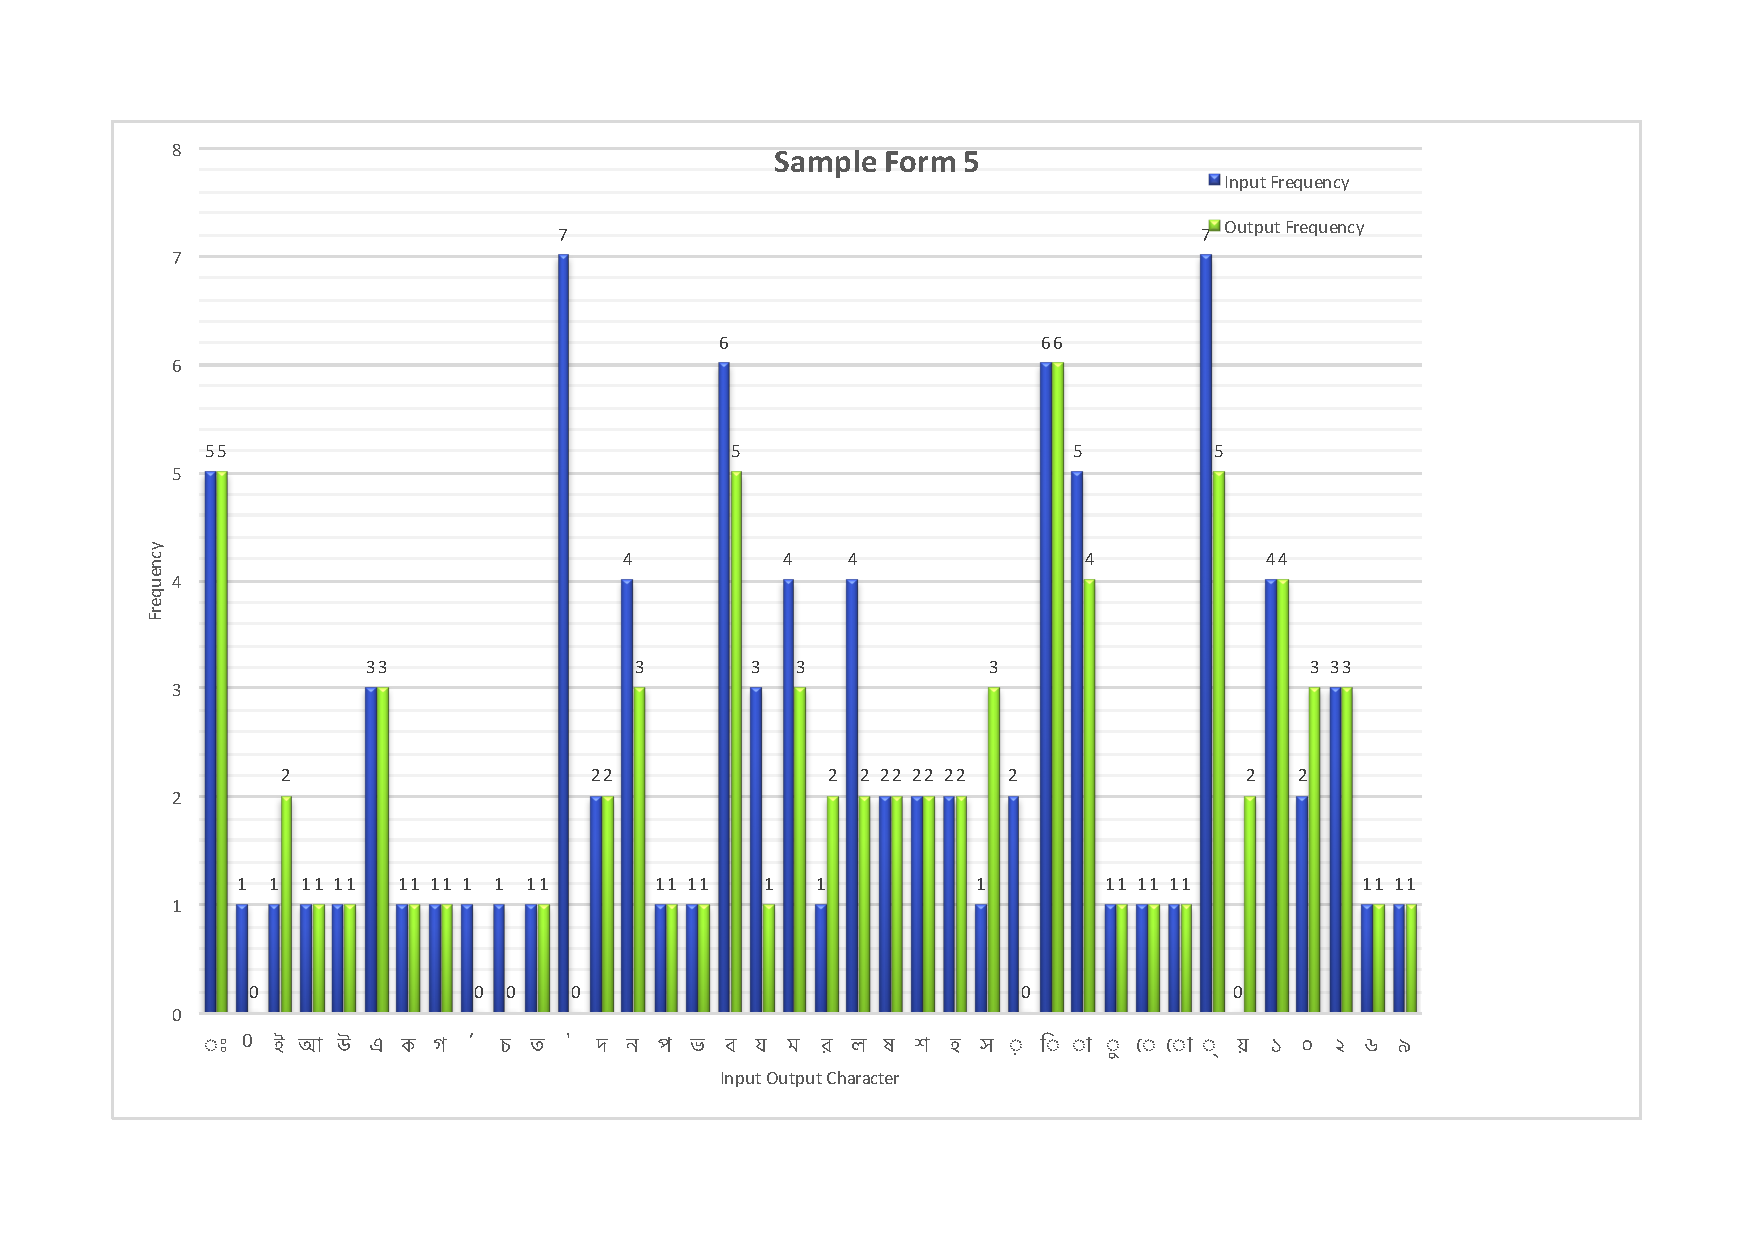
\includegraphics[width=1\textwidth]{Bform5.pdf}
\caption {Bar chart Input Output Frequency of Sample form 5}
\label {fig:Bbar5}
\end{figure}

According to these output of bangla from, we can say that here accuracy of our bangla tarining data upto 75\%. In our training data big problem is with complex bangla word. Our trained tesseract can't detect complex bangla word perfectly.
